\tikzset{every picture/.style={line width=0.75pt}} %set default line width to 0.75pt        

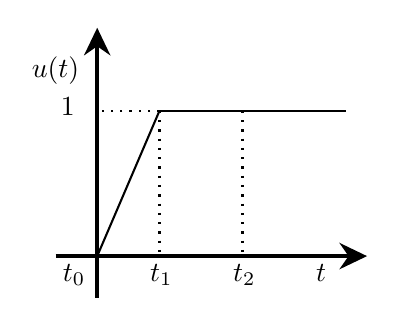
\begin{tikzpicture}[x=0.75pt,y=0.75pt,yscale=-1,xscale=1]
	%uncomment if require: \path (0,300); %set diagram left start at 0, and has height of 300
	
	%Straight Lines [id:da2875292600189103] 
	\draw [line width=1.5]    (100,160) -- (100,34) ;
	\draw [shift={(100,30)}, rotate = 450] [fill={rgb, 255:red, 0; green, 0; blue, 0 }  ][line width=0.08]  [draw opacity=0] (13.4,-6.43) -- (0,0) -- (13.4,6.44) -- (8.9,0) -- cycle    ;
	%Straight Lines [id:da3046472264214819] 
	\draw [line width=1.5]    (80,140) -- (226,140) ;
	\draw [shift={(230,140)}, rotate = 180] [fill={rgb, 255:red, 0; green, 0; blue, 0 }  ][line width=0.08]  [draw opacity=0] (13.4,-6.43) -- (0,0) -- (13.4,6.44) -- (8.9,0) -- cycle    ;
	%Straight Lines [id:da9835771066030095] 
	\draw [line width=0.75]    (100,140) -- (130,70) ;
	%Straight Lines [id:da7083475840908604] 
	\draw [line width=0.75]    (130,70) -- (220,70) ;
	%Straight Lines [id:da20127916146270386] 
	\draw  [dash pattern={on 0.84pt off 2.51pt}]  (130,70) -- (130,140) ;
	%Straight Lines [id:da677805480574649] 
	\draw  [dash pattern={on 0.84pt off 2.51pt}]  (130,70) -- (100,70) ;
	%Straight Lines [id:da35275281353074295] 
	\draw  [dash pattern={on 0.84pt off 2.51pt}]  (170,70) -- (170,140) ;
	
	% Text Node
	\draw (81,62.4) node [anchor=north west][inner sep=0.75pt]    {$1$};
	% Text Node
	\draw (82,142.4) node [anchor=north west][inner sep=0.75pt]    {$t_0$};
	% Text Node
	\draw (124,142.4) node [anchor=north west][inner sep=0.75pt]    {$t_{1}$};
	% Text Node
	\draw (164,142.4) node [anchor=north west][inner sep=0.75pt]    {$t_{2}$};
	% Text Node
	\draw (67,42.4) node [anchor=north west][inner sep=0.75pt]    {$u(t)$};
	% Text Node
	\draw (204,142.4) node [anchor=north west][inner sep=0.75pt]    {$t$};
	
	
\end{tikzpicture}